
\subsection{Funzionamento LED}
Un led è un diodo che emette luce quando attraversato da una corrente. Il diodo è in grado di fare ciò grazie ad una giunzione PN.\\
Una giunzione PN è una giunzione tra 2 materiali semicontrollori drogati in maniera opposta. Da un lato il materiale è drogato con atomi che hanno un elettrone debolmente legato, mentre l'altra parte è drogata con atomi che hanno un elettrone in meno.\\
Questa asimmetria della componente permette al diodo di avere un comportamento diverso a seconda della direzione della corrente.\\ 

\pagebreak
\begin{wrapfigure}{r}{0.4\linewidth}
    \centering
    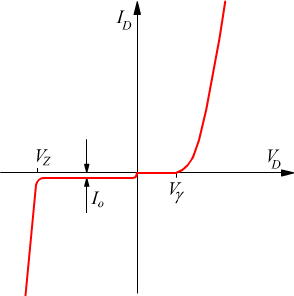
\includegraphics[width=\linewidth]{photomultiplier/assets/shokley.png}
    \caption{Legge di Shockley per il comportamento ideale del diodo}
    \label{fig:Photomultiplier}
\end{wrapfigure}

Quindi, se la corrente è diretta in un senso, detta \textit{polarizzazione diretta}, il diodo si comporta come un corto circuito. Se la corrente è diretta nell'altro senso, detta \textit{polarizzazione inversa}, il diodo si comporta come un circuito aperto.\\

In particolare, se polarizzato direttamente, può capitare che degli elettroni si mischino con le lacune cancellandosi a vicenda. L'energia mancante viene emessa come fotone con la stessa energia dell'elettrone.\\
L'energia dell'elettrone, e quindi la frequenza del fotone emesso, dipendono dalla giunzione PN e dai materiali che la compongono. Questo significa che, cambiando i materiali, si può cambiare la frequenza della luce emessa.\\

\subsection{Funzionamento Fotomoltiplicatore}
Con lo stesso principio del LED, ma in polarizzazione inversa, siamo in grado di creare un fotomoltiplicatore. Ovvero uno strumento che, se colpito da un fotone, emette un elettrone e quindi crea una corrente nel circuito.\\

Perchè questo succeda però, l'elettrone (e quindi la lacuna) creata con il fotone, deve avere abbastanza energia per uscire dal diodo e iniziare a scorrere nel circuito. Per questo serve aumentare il voltaggio. Una volta aumentato il voltaggio, però gli elettroni possono avere abbastanza energia per colpire altri atomi e creare altri elettroni, a creare una valanga. La tensione necessaria per creare questo fenomeno è detta \textit{tensione di breakdown}.\\

Così facendo, possiamo collegare una tensione all'interno del circuito con l'urto di un fotone con il fotomoltiplicatore.\\